\begin{figure}[htbp]
\centering 
  \subfloat[Parameter space plot, \acs{SCT}, $\sigma_n=1068$ Pa, P=1.0.]{
	  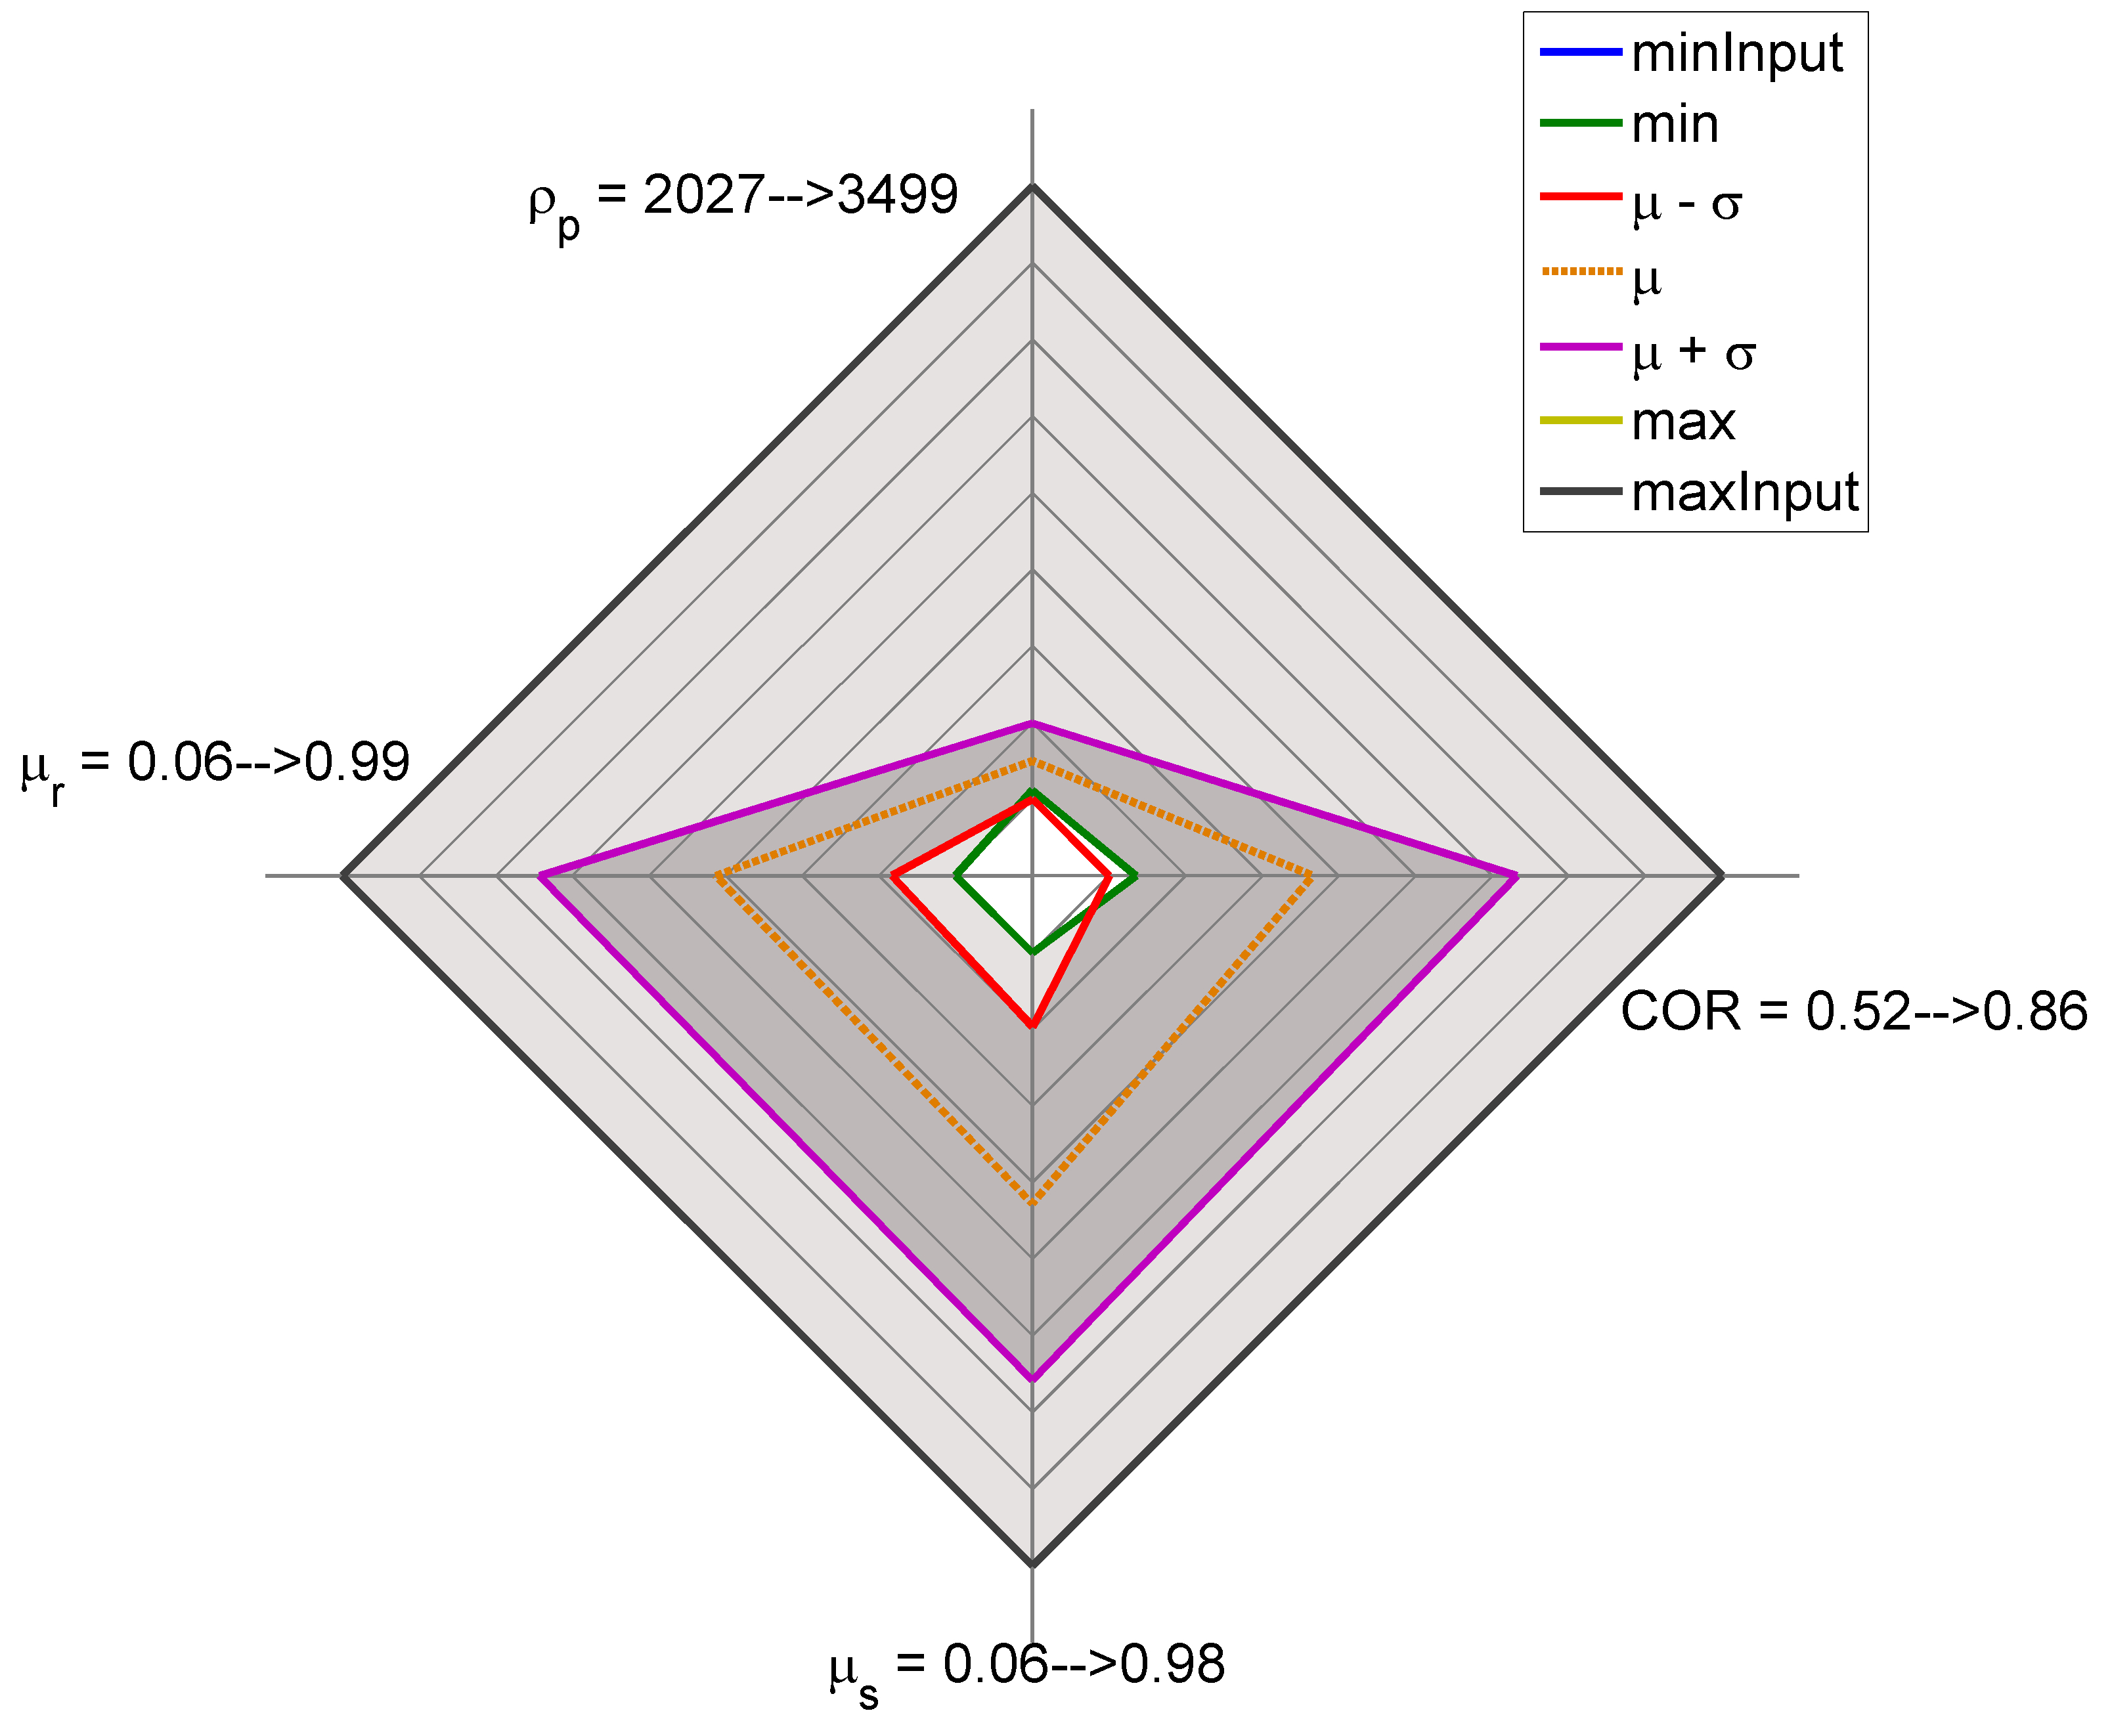
\includegraphics[width=.35\columnwidth]{images/041radarpirker1schulze1068}
	  \label{fig:041radarpirker1schulze1068}
  }
  \\
    \subfloat[Parameter space plot, \acs{SCT}, $\sigma_n=10070$ Pa, P=0.8.]{
	  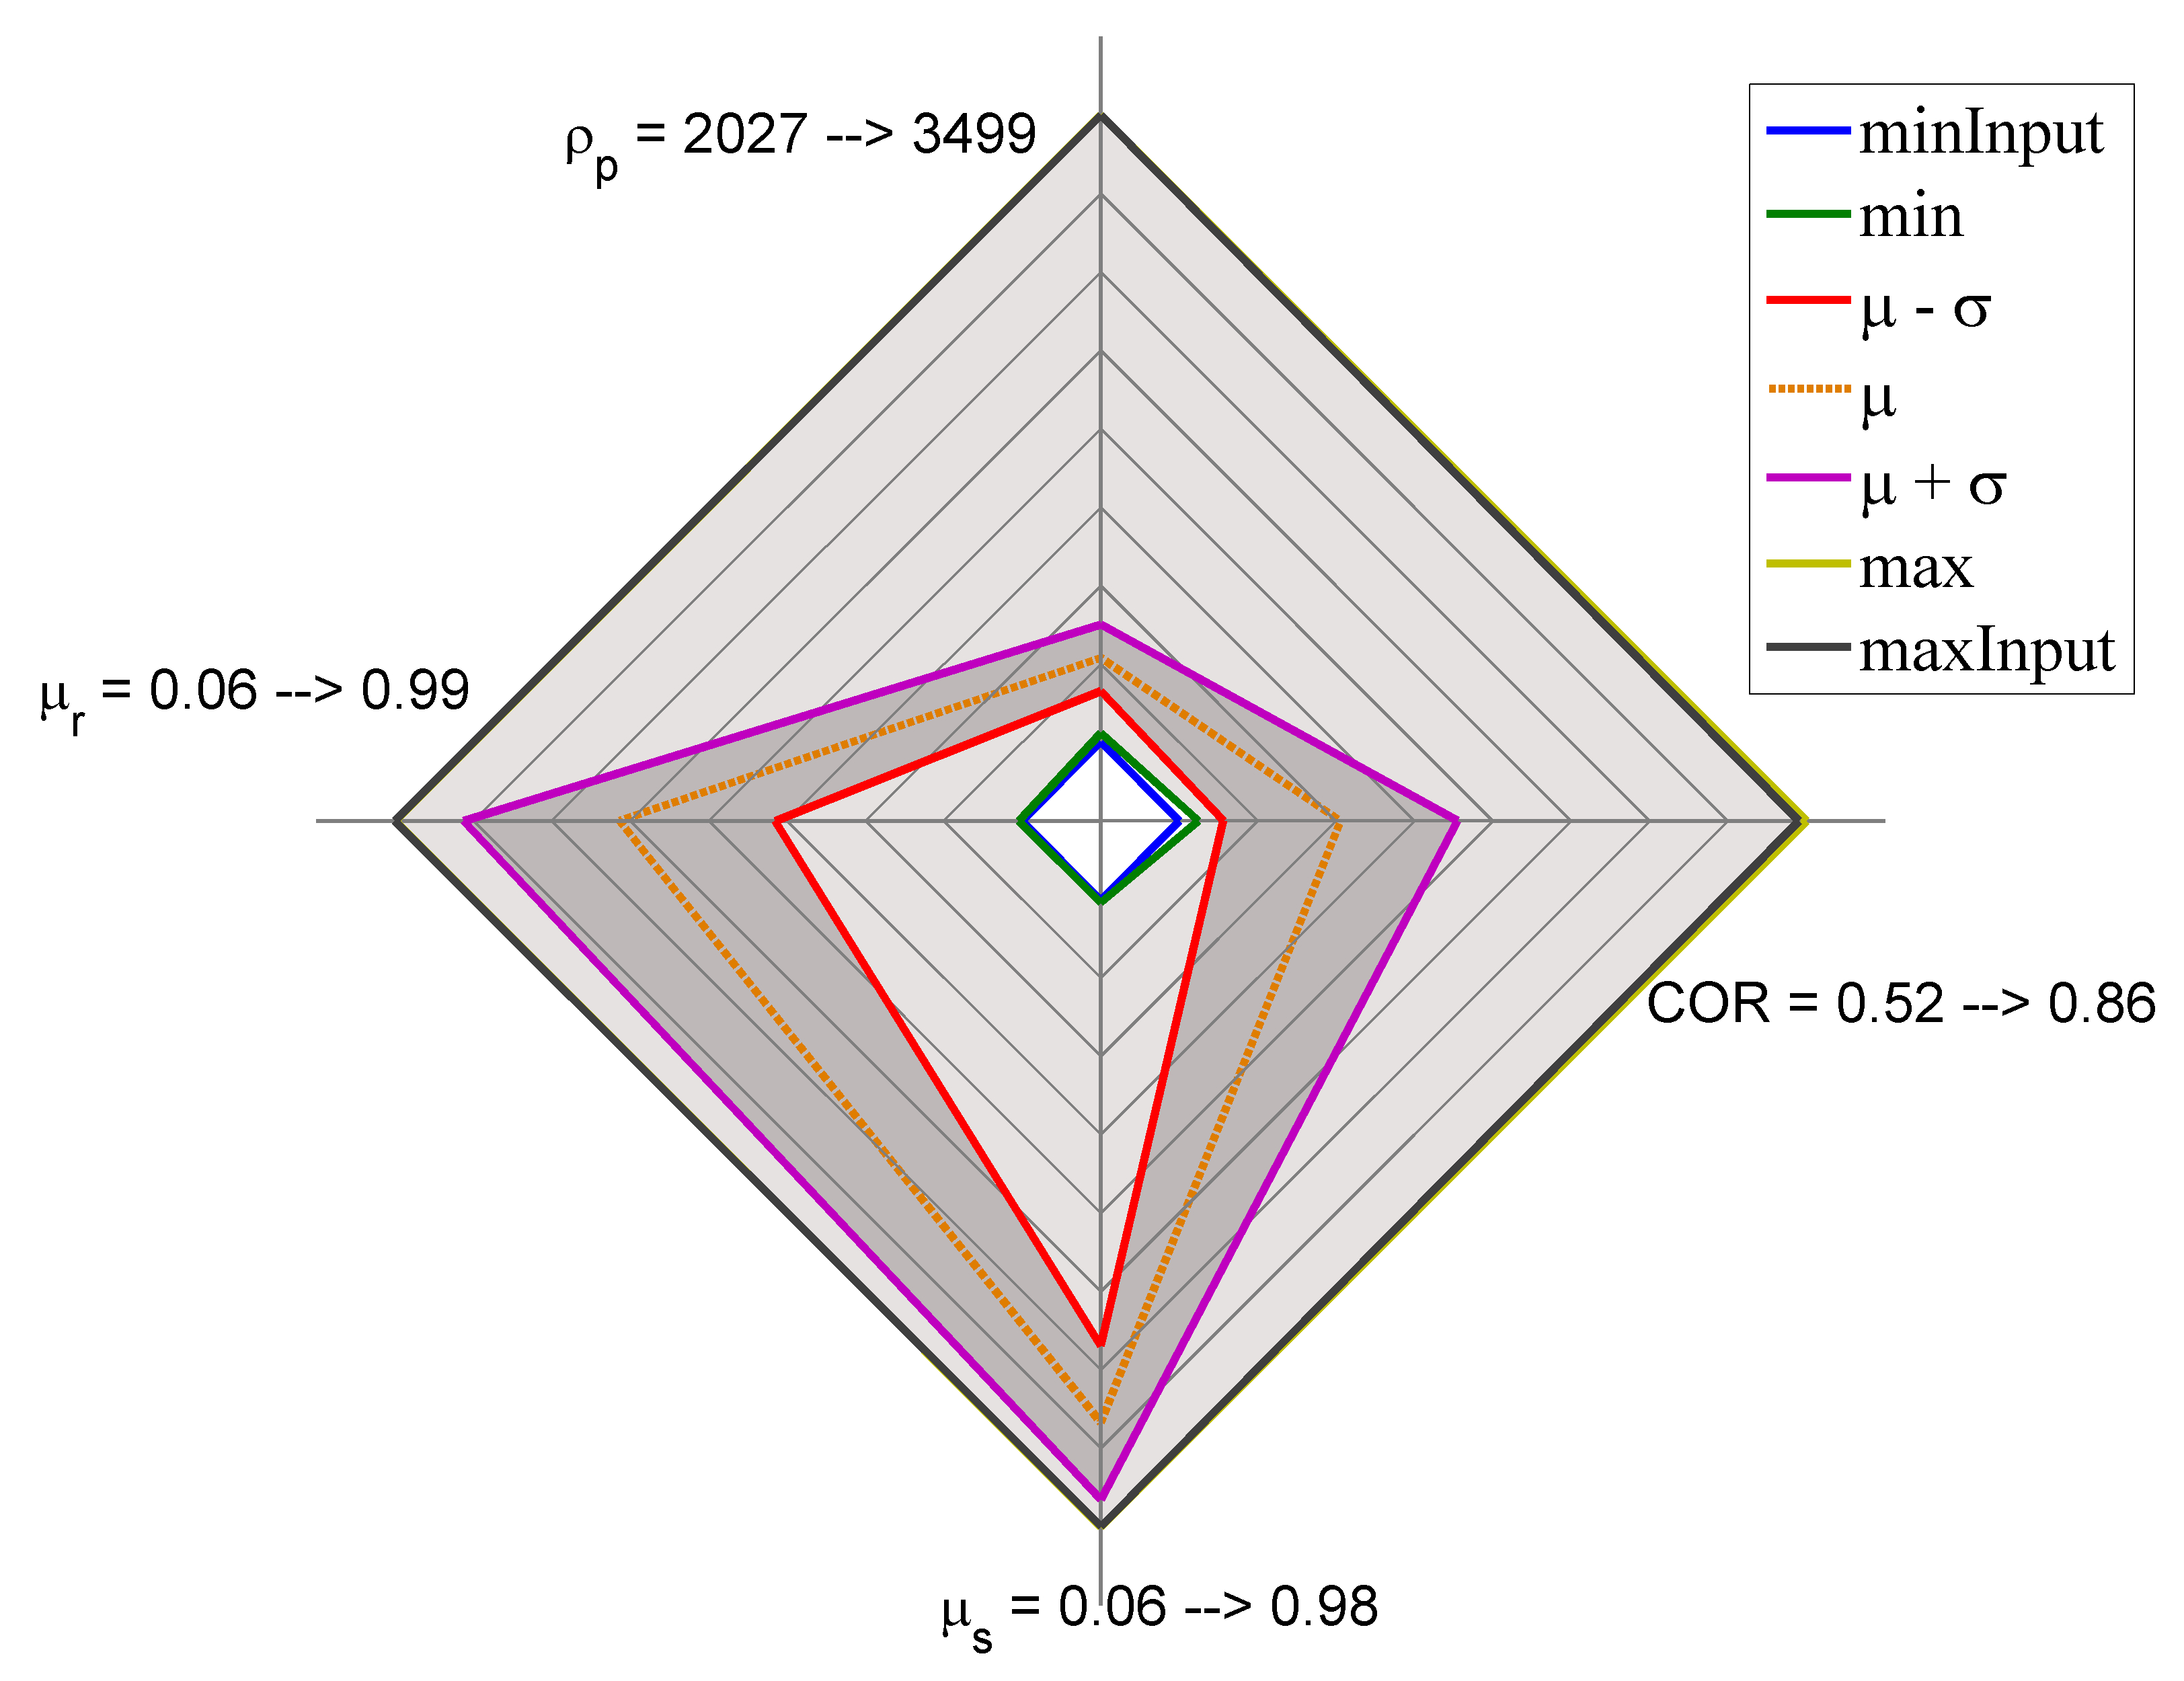
\includegraphics[width=.35\columnwidth]{images/026radarpirker08schulze10070}
	  \label{fig:026radarpirker08schulze10070}
  }
  \\
  \subfloat[Parameter space plot, \acs{SCT}, $\sigma_n=10070$ Pa, P=1.0.]{
	  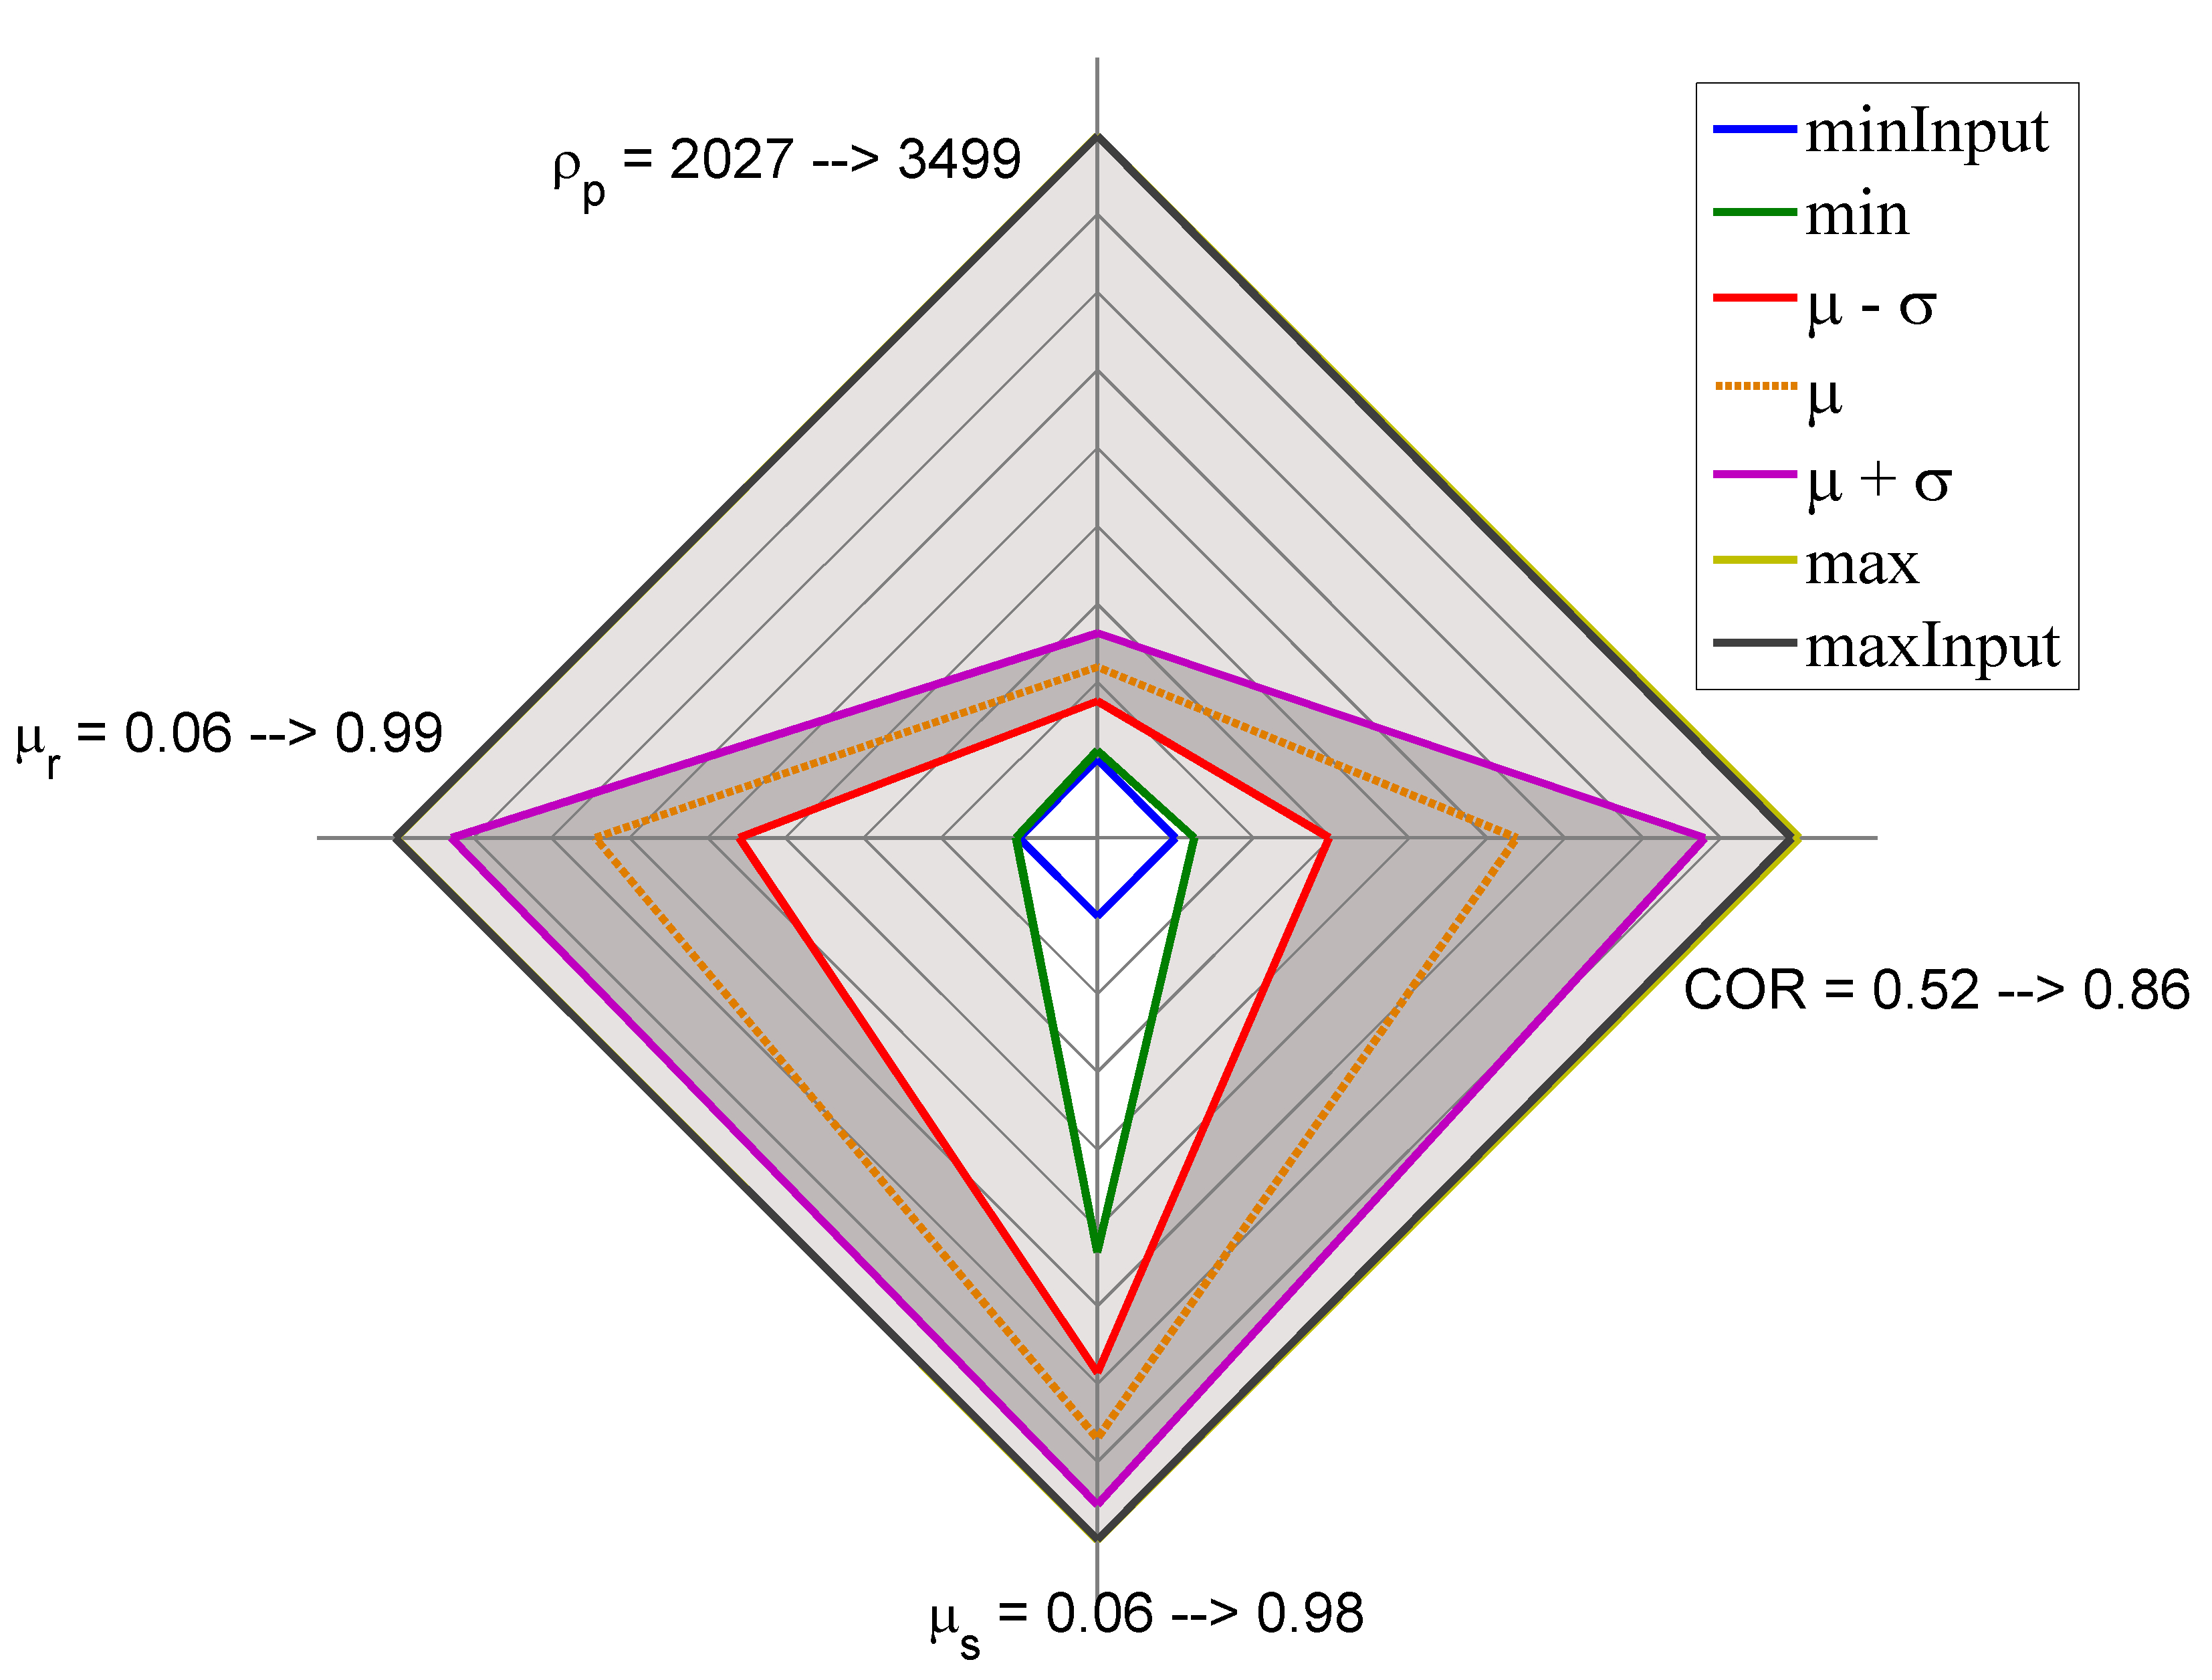
\includegraphics[width=.35\columnwidth]{images/024radarpirker1schulze10070}
	  \label{fig:024radarpirker1schulze10070}
  }
  \quad
    \subfloat[Box plot, \acs{SCT}, $\sigma_n=10070$ Pa, P=1.0.]{
	  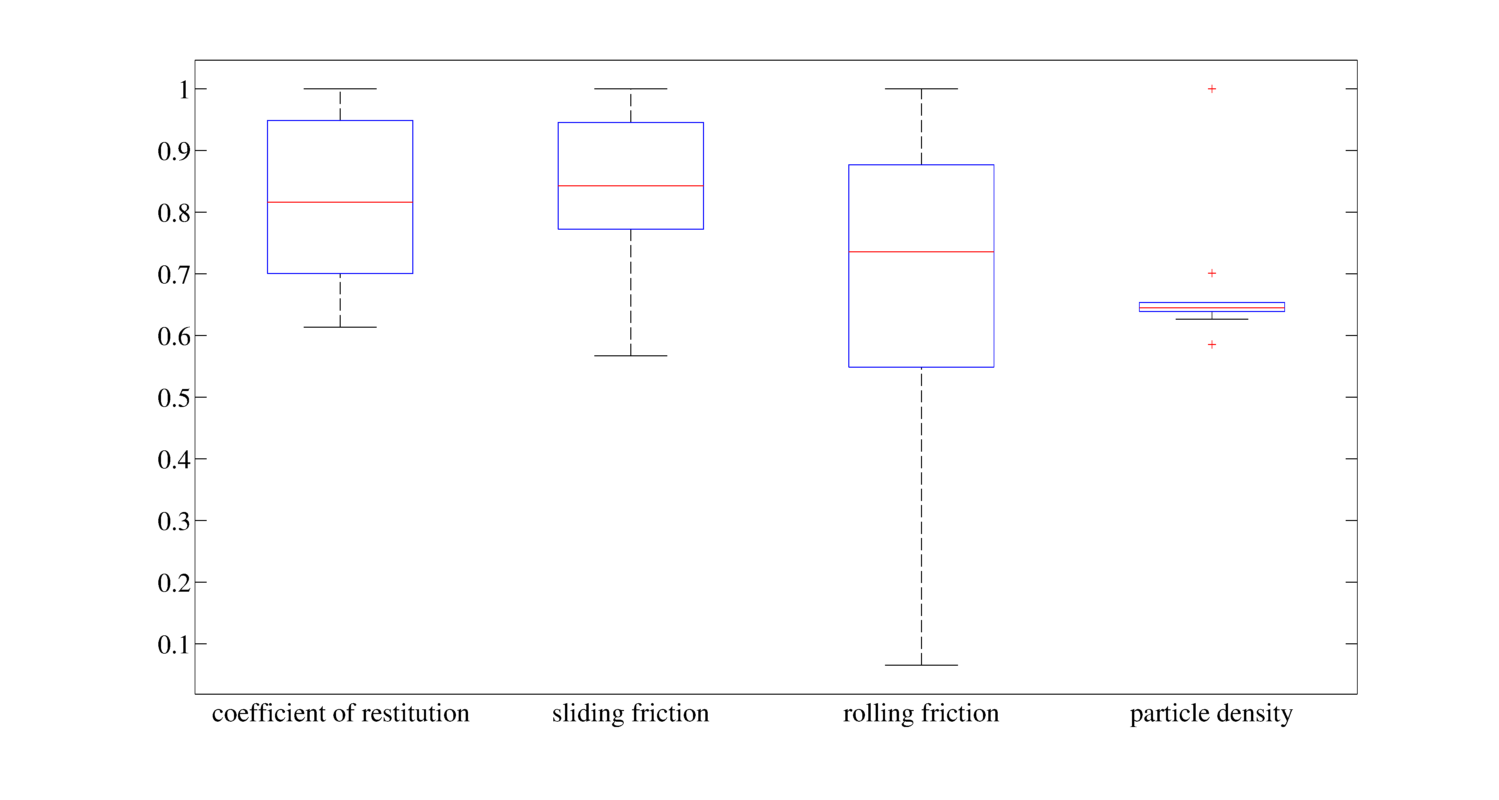
\includegraphics[width=.35\columnwidth]{images/075sctboxplot}
	  \label{fig:075sctboxplot}  }
  \\
    \subfloat[Parameter space plot, \acs{SCT}, $\sigma_n=10070$ Pa, P=1.2.]{
	  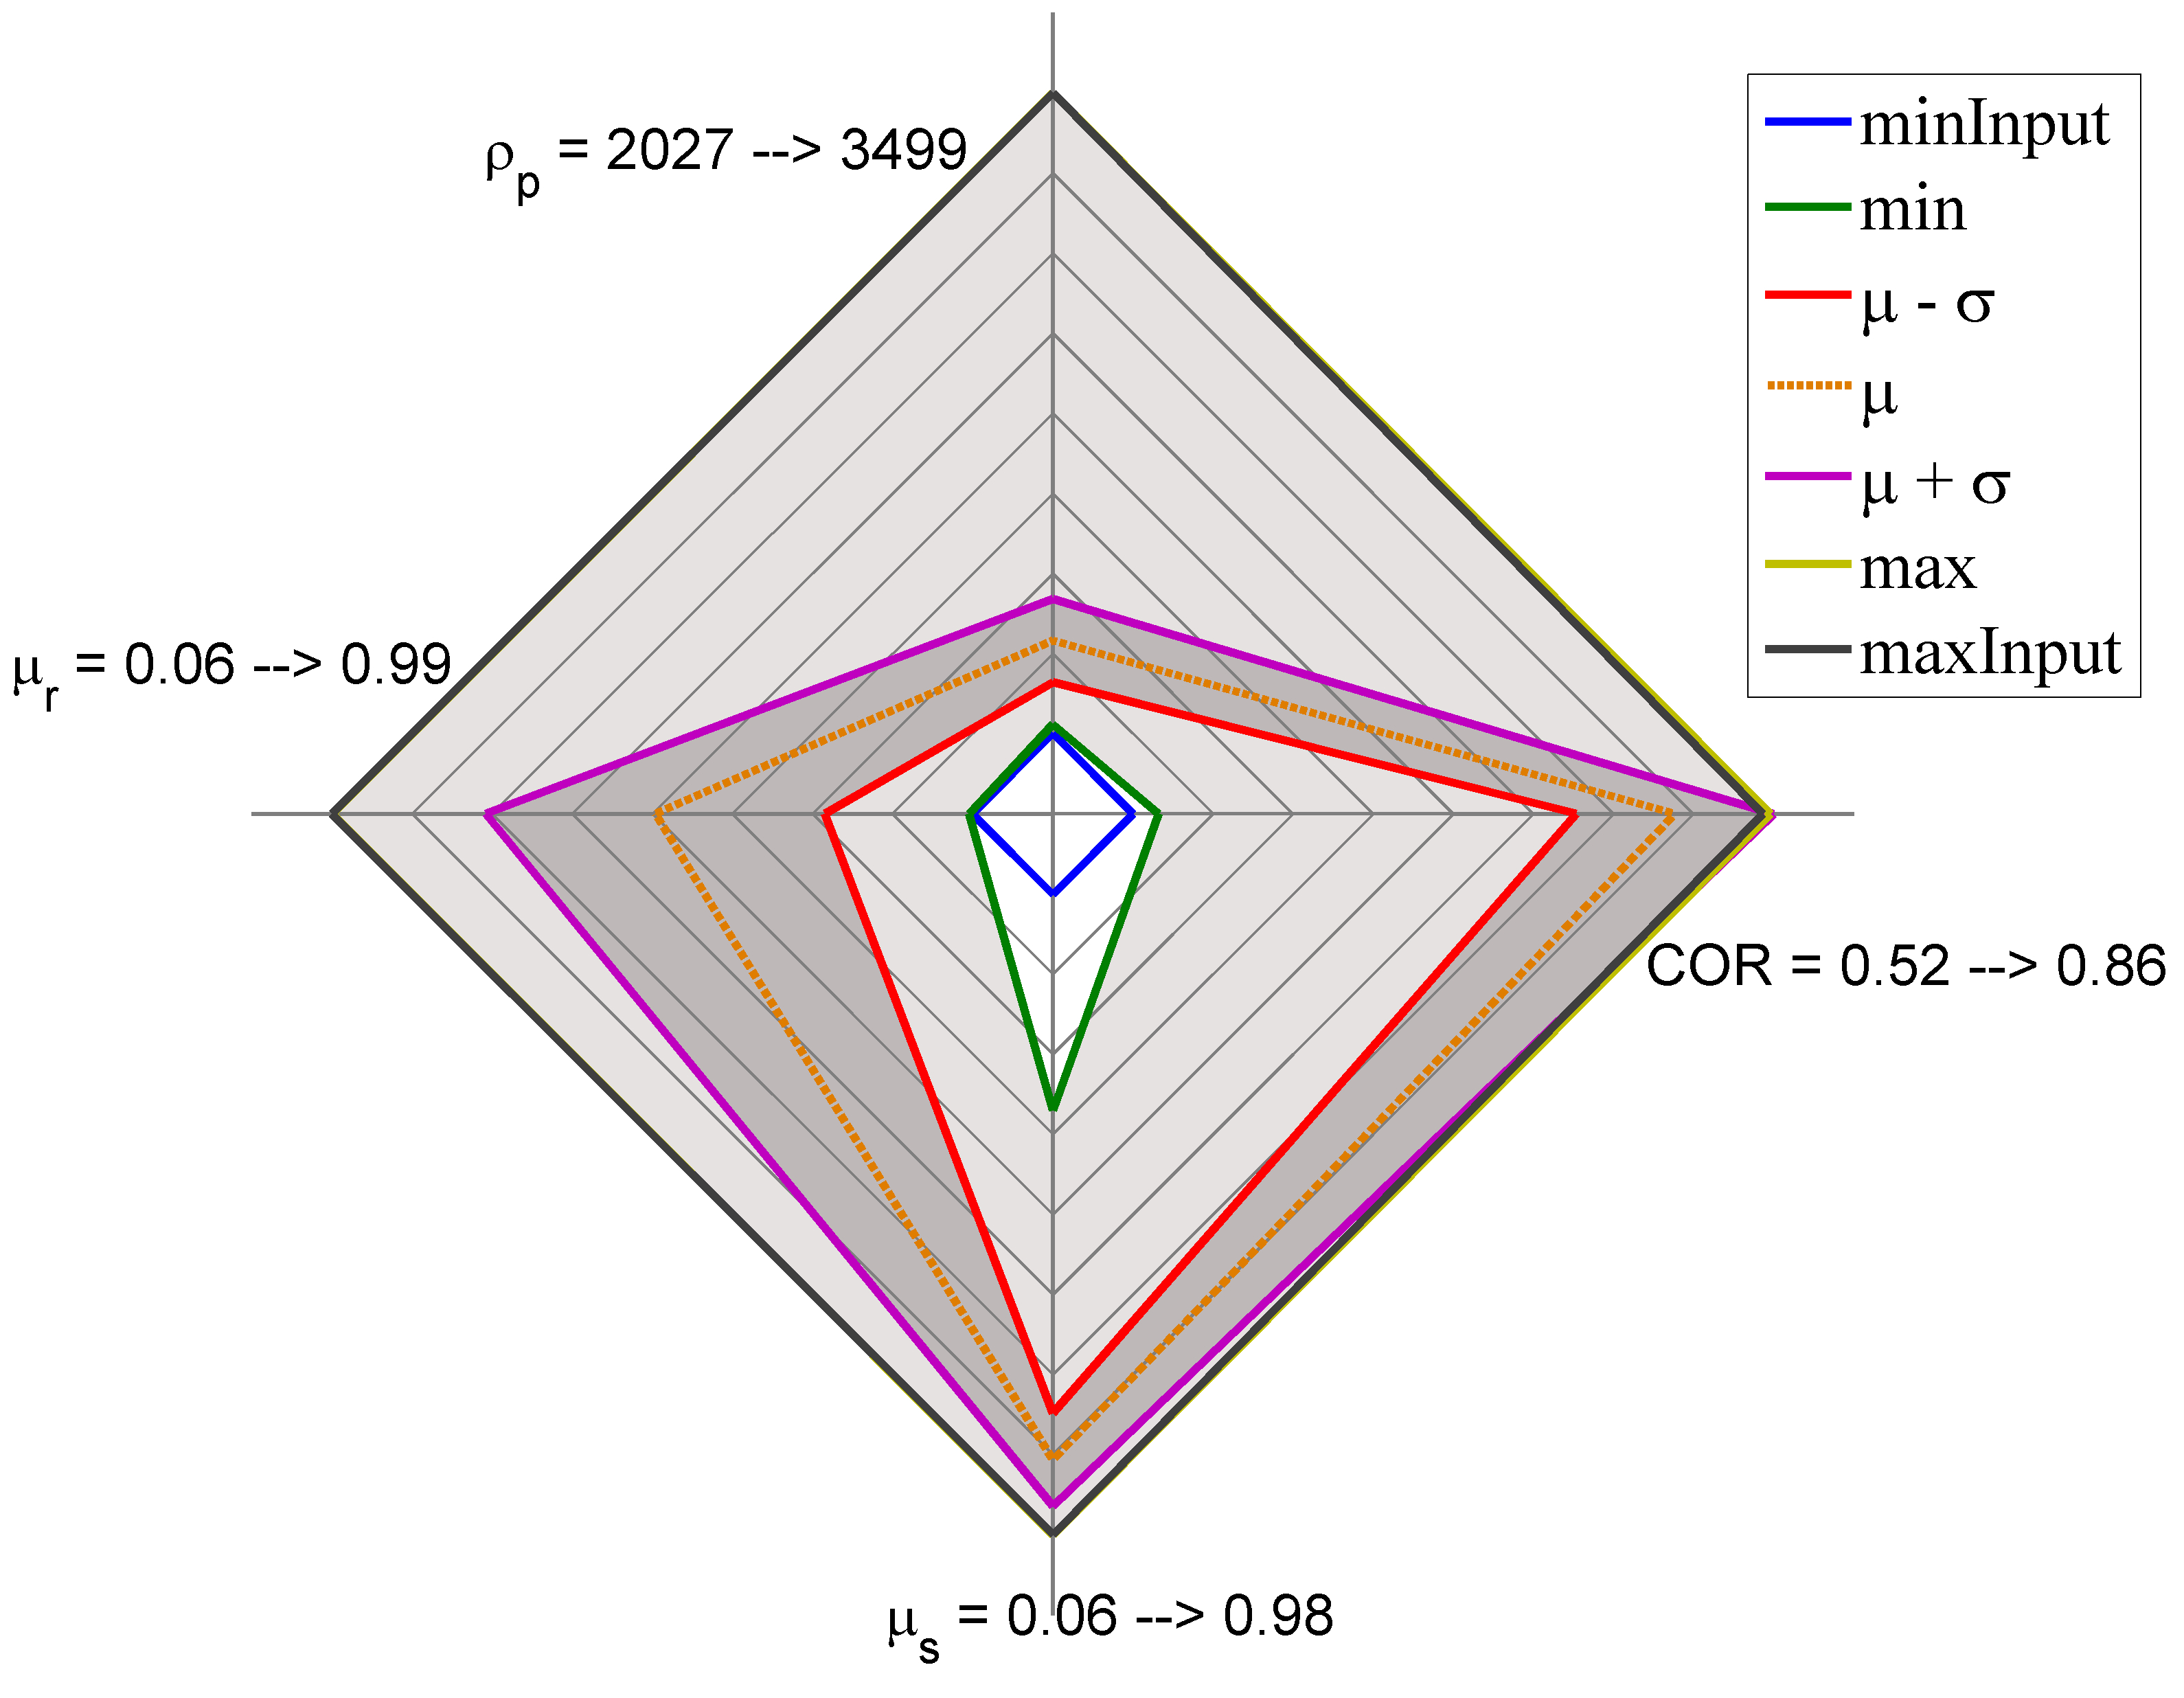
\includegraphics[width=.35\columnwidth]{images/028radarpirker12schulze10070}
	  \label{fig:028radarpirker12schulze10070}
  }
  \caption{SCT parameter space plots.}
  \label{fig:079sctparameterspaceplots}
\end{figure}